\chapter[Fundamentação Teórica]{Fundamentação Teórica}
\label{cp:fundamentacao}

\section{Gerenciamento de Projetos}
\label{sec:gerenciamento_de_projetos}

\subsection{Modelo Tradicional}
\label{sec:modelo_tradicional}

Uma metodologia de gerenciamento de projetos no modelo tradicional, de acordo com \cite{kerzner} é o alcance da excelência no gerenciamento de projetos se torna impossível sem um processo repetitivo que possa ser utilizado em cada projeto.

No modelo tradicional, um dos mais modelos mais utilizados é o RUP \textit{(Rational Unified Process)}. O RUP oferece uma metodologia responsável por responder questões como boas práticas para o gerenciamento de projetos, com o objetivo de estruturar e formatar os processos associados às atividades que envolvem a tecnologia de informação. 

As 4 fases principais do RUP podem ser vistas na figura \ref{img:fases_do_rup}:

\begin{figure}[H]
	\centering
	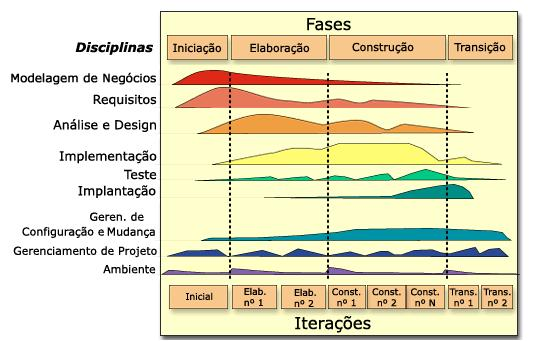
\includegraphics[width=0.8\textwidth]{figuras/fases_rup.jpg}
	\caption{Fases do RUP. Fonte: \cite{rup}.}
	\label{img:fases_do_rup}
\end{figure}

O desenvolvimento do plano de gerenciamento do projeto é uma atividade iterativa ao longo do ciclo de vida do projeto, sempre pronto para melhoria contínua e permitindo à equipes do projeto definir e trabalhar com maior nível de detalhes. De acordo com o \cite{pmbok}, as fases do \cite{rup} são sobrepostas, ou seja, o início de uma fase é ao término de uma outra, isso leva a algumas atividades ocorrerem de forma paralela. A maneira como este tipo de projeto aumenta os riscos, retrabalhos, e exigir recursos adicionais para permitir as atividades em paralelo, como mostrado na figura \ref{img:fases_do_rup}.

Nesta perspectiva, se tem o papel do gerente de projeto como um líder responsável por liderar a equipe para alcançar os objetivos previstos no planejamento do projeto. Entre as funções destes líderes se tem:

\begin{itemize}
    \item Conhecimento acerca do gerenciamento de projetos;
    \item Desempenho para aplicar seus conhecimentos na prática;
    \item Comportamento pessoal de liderança, atingindo objetivos e equilibrando restrições.
\end{itemize}

Este tipo de gerenciamento de projeto é mais utilizado em empresas já consolidadas, de ramo mais formal, que possui mais burocracia em seus projetos e por tanto maior rigor de documentação e de liderança dos gerentes de projeto. Essa hierarquia pode ser vista na Figura \ref{img:gerencia_de_projetos_tradicional}.

\begin{figure}[H]
	\centering
	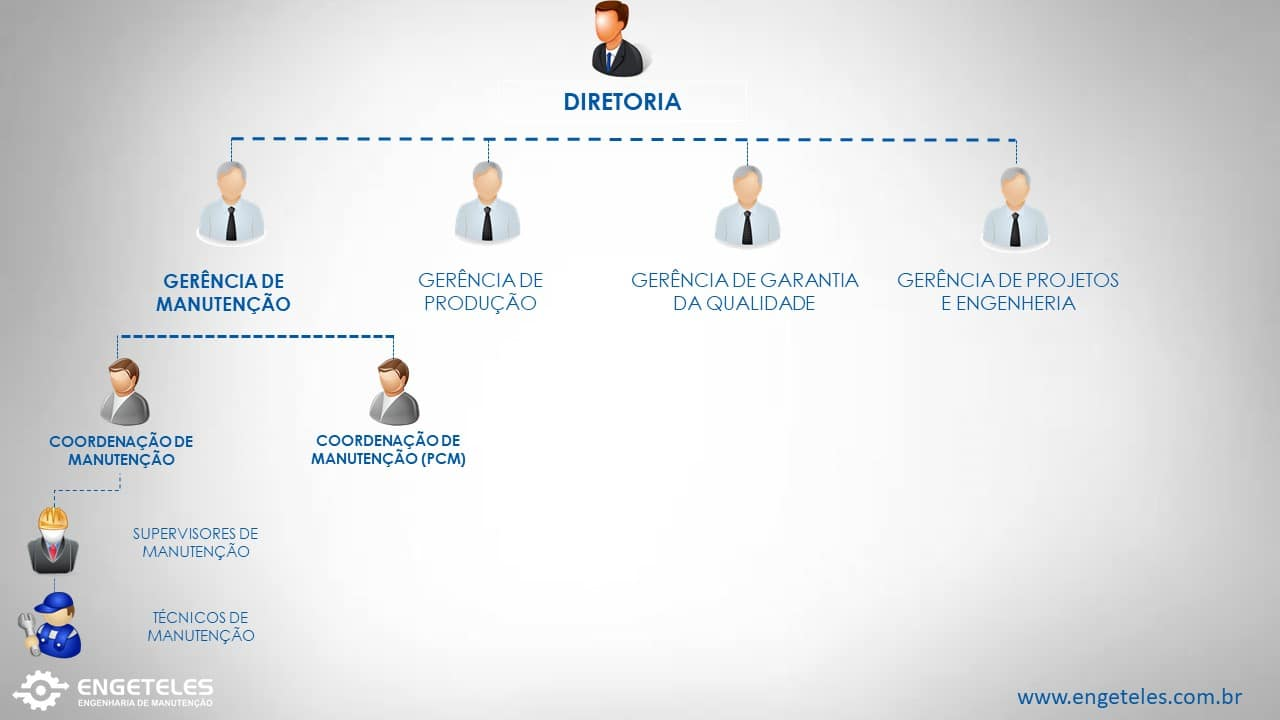
\includegraphics[width=0.8\textwidth]{figuras/gerencia_de_projeto.jpg}
	\caption{Hierarquia em projetos tradicionais. Fonte: \cite{gerentes_tradicionais}.}
	\label{img:gerencia_de_projetos_tradicional}
\end{figure}

\subsubsection{Casos de Uso}
\label{sec:casos_de_uso}

Os casos de uso é uma das principais características presentes na linguagem de modelagem UML (unified modeling language), ou linguagem modelada unificada. \cite{sommerville} define os objetivos dos casos de uso são de identificar os atores envolvidos e dá o nome ao tipo de interação. Os casos de uso é um diagrama de auto nível, ou seja, de fácil entendimento para o usuário final que possui os objetivos mais amplos de auxiliar a comunicação entre cliente e analistas, e apresentar as principais funcionalidades do sistema com foco no cliente.

Na Figura \ref{img:exemplo_caso_de_uso} é possível visualizar um exemplo de caso de uso:

\begin{figure}[H]
	\centering
	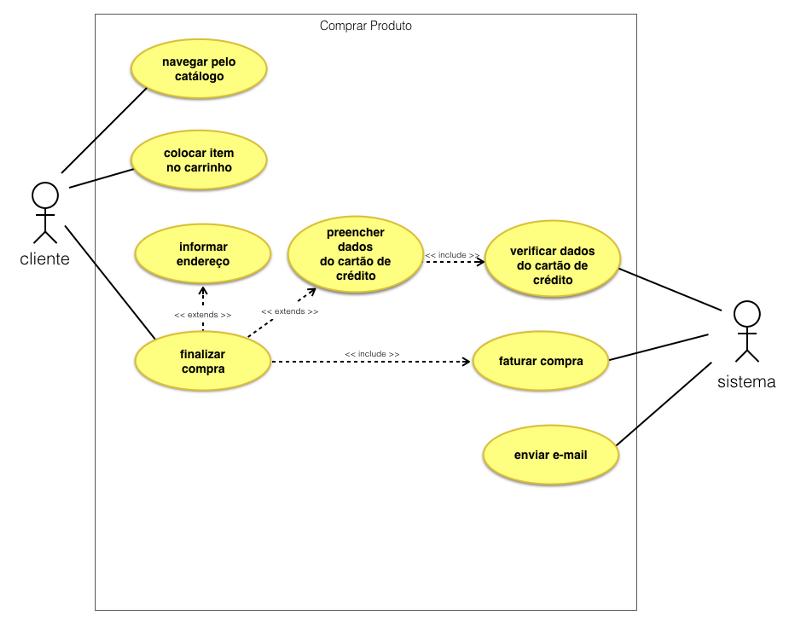
\includegraphics[width=1.0\textwidth]{figuras/caso_de_uso_exemplo.png}
	\caption{Exemplo de Caso de Uso. Fonte: \cite{casos_de_uso}.}
	\label{img:exemplo_caso_de_uso}
\end{figure}

\subsection{Modelo Ágil}
\label{sec:modelo_agil}

Em contraposição ao modelo tradicional, surte o manifesto ágil como uma reação contra o processo burocrático presente no modelo tradicional, que possuem por característica atividades sequências em modelo cascata. Segundo a \cite{chaos} apenas 16,2\% dos projetos entregues por companhias americanas foram entregues respeitando prazos, custos previamente acordados e objetivos determinados. Segundo a própria \cite{chaos}, as principais causas destes problemas estavam relacionadas com o modelo sequencial tradicional.

O modelo ágil, segundo \cite{soares}, ela deve primeiro aceitar as mudanças em vez de tentar prevê-las, agir de maneira rápida sabendo receber, avaliar e responder como elas devem ser respondidas. As principais características da metodologia ágil são:

\begin{itemize}
	\item Desenvolvimento iterativo e incremental;
	\item Comunicação;
	\item Documentação extensiva; 
\end{itemize}

Em 2001, membros da comunidade de \textit{software} se reuniram e criaram o \cite{agile_manifest}. O objetivo deste manifesto é utilizar as melhores práticas observadas em projetos anteriores que obtiveram sucessos.

Os principais conceitos do manifesto ágil são:

\begin{itemize}
	\item Indivíduos e interações ao invés de processos e ferramentas;
	\item \textit{Software} executável ao invés de documentação;
	\item Colaboração do cliente ao invés de negociação de contratos;
	\item Resposta rápida a mudanças ao invés de seguir planos pré-estabelecidos.
\end{itemize}

No modelo ágil os requisitos dos clientes podem ser mudados a qualquer momento, e o time de gerência e desenvolvimento devem estar preparados para conversar com o cliente a fim de resolver as alterações de requisitos da melhor maneira possível. Este tipo de pensamento no modelo tradicional é mais difícil de acontecer, pois ao observar a figura \ref{img:fases_do_rup}, é possível notar ao iniciar uma fase, essa mesma fase não é retornada mais tarde, ou seja, no modelo tradicional uma troca de requisitos pode levar ao reinicio do projeto.

Este modelo é mais focado para empresas emergentes, que não são muito rigorosas em seus processos e aceita que mudanças nos requisitos ou na visão do produto são sempre bem vindas, desde que melhore o projeto final.

\subsubsection{Scrum}
\label{sec:scrum}

Uma das boas práticas adotadas ao modelo ágil é o \textit{Scrum}. O \textit{Scrum}, é um \textit{framework} que se refere ao jogo \textit{Rugby}, que é a ação dos jogadores se organizarem em círculo para planejar a próxima jogada. Um dos principais pontos de vista do \textit{Srum} é mostrar um projeto com pequenos ciclos, aumentando as iterações entre os participantes, mas com visão a longo prazo.

O ciclo de vida pode ser visto na figura \ref{img:ciclo_de_vida_scrum}:

\begin{figure}[H]
	\centering
	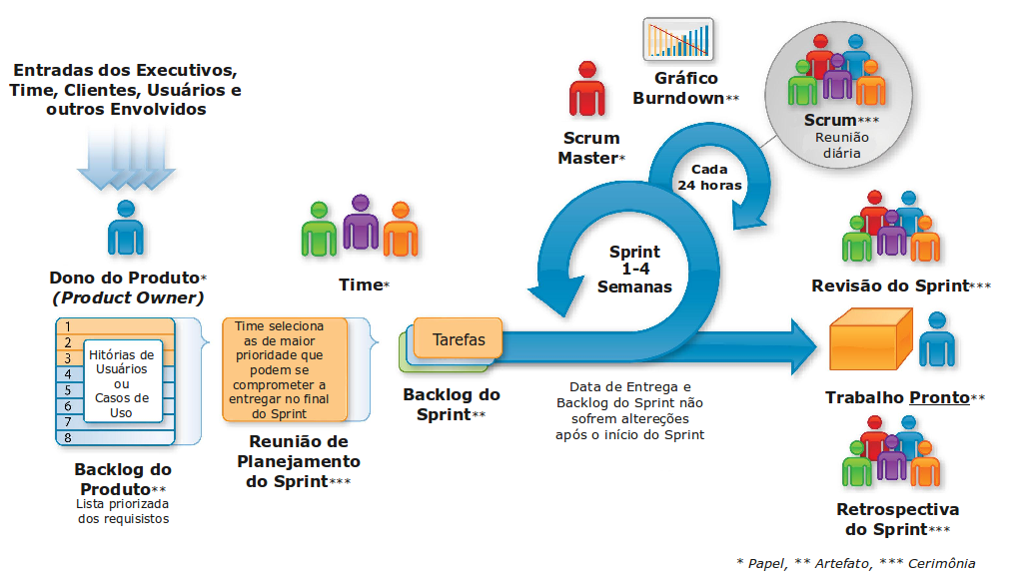
\includegraphics[width=0.8\textwidth]{figuras/ciclo_de_vida_scrum.png}
	\caption{Ciclo de Vida SCRUM. Fonte: \cite{scrum}.}
	\label{img:ciclo_de_vida_scrum}
\end{figure}

Como visto na figura \ref{img:ciclo_de_vida_scrum}, o \textit{Scrum} é um ciclo progressivo de várias iterações bem definidas, denominadas \textit{Sprints}. As \textit{Sprints} podem ter duração de uma a quatro semanas. Antes de cada \textit{Sprint}, deve ser realizada a reunião de planejamento da \textit{Sprint}, chamada de \textit{Sprint Planning Meeting}. A \textit{Sprint Planning Meeting} é uma reunião de planjemanto em que o \textit{Product Owner}
prioriza os itens do \textit{Product Backlog} e a equipe seleciona as atividades que serão implementadas ao longo da \textit{Sprint}. No \textit{Product Backlog} são registradas as funcionalidades que serão implementadas pedidas pelo \textit{Product Backlog}. 

Com o objetivo de saber o progresso de cada equipe dentro da \textit{Sprint}, ocorrem as reuniões diárias, denominadas \textit{Daily Meetings}, que tem duração de no máximo 15 minutos e ocorrem com todos os participantes em pé, respondendo perguntas como: "O que você fez ontem?", "O que você fez hoje?" e "O que você vai fazer amanhã?". 

Ao final de uma \textit{Sprint} é feita uma análise gráfico do progresso do projeto atráves do \textit{Sprint Backlog} durante a \textit{Sprint Review}. Após a \textit{Sprint Review} ocorre a \textit{Sprint Retrospective} que é a análise de experiências que ocorreram durante a \textit{Sprint} sejam boas ou não a fim de melhora-las.

Segundo \cite{fowler}, as equipes devem possuir um quadro para registro das atividades, denominado \textit{Kanban}. O \textit{Kanban} possui o objetivo de auxiliar as equipes em relação ao progresso da \textit{Sprint}, esse quadro pode ser dividido em 4 fases:

\begin{itemize}
	\item Para fazer;
	\item Em andamento (com o nome do responsável pela atividade);
	\item Em revisão;
	\item Feito.
\end{itemize}

\begin{figure}[H]
	\centering
	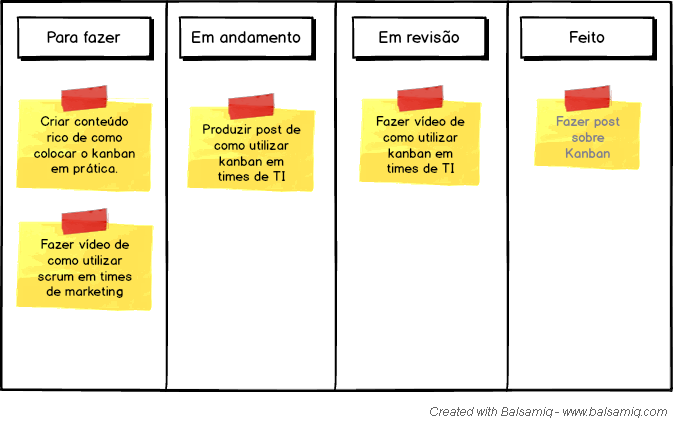
\includegraphics[width=1.0\textwidth]{figuras/kanban.png}
	\caption{Quadro Kanban. Fonte: \cite{kanban}.}
	\label{img:kanban}
\end{figure}

O \textit{Scrum} possui seus papéis bem definidos, podendo ser alterados ao longo do desenvolvimento do projeto. Esses papéis podem ser vistos na figura \ref{img:papeis_scrum}.

\begin{figure}[H]
	\centering
	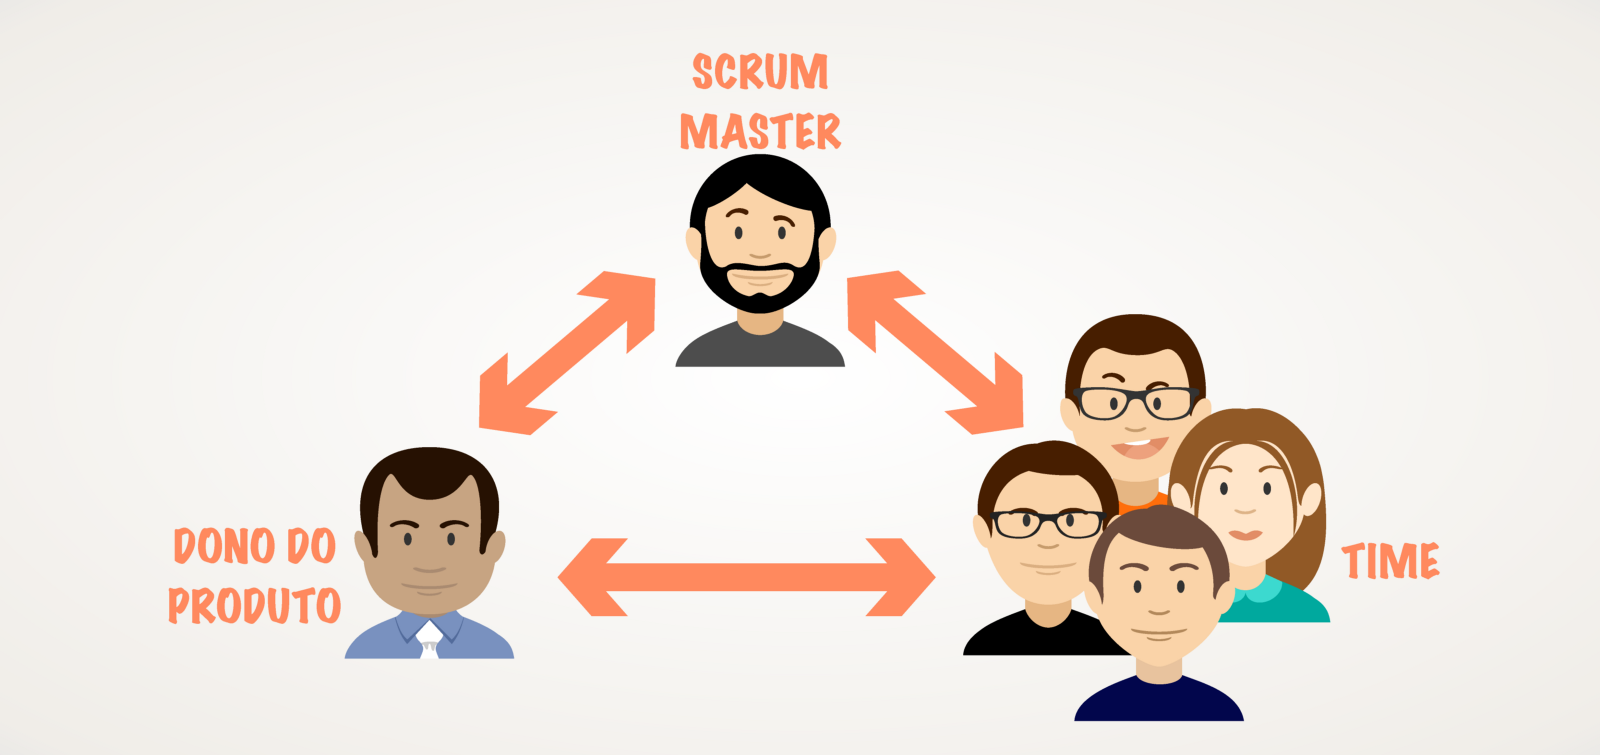
\includegraphics[width=1.0\textwidth]{figuras/papeis_scrum.png}
	\caption{Papéis Scrum. Fonte: \cite{papeis_scrum}.}
	\label{img:papeis_scrum}
\end{figure}

Como observado na figura \ref{img:papeis_scrum}, o \textit{Scrum} possui três papéis bem definidos: o \textit{Product Owner}, conhecido como PO, o \textit{Scrum Master} e por fim temos o \textit{Dev Team}. 

\subsubsubsection{Product Owner}

O \textit{Product Owner}, é o dono do produto. É ele que fornece o conhecimento do negócio em forma de requisitos para a equipe e na forma pratíca são os patrocionadores/clientes do produto. O PO organiza e prioriza o \textit{Product Backlog} (que são os itens que devem ser desenvolvidos), esse papel deve ser assumido por pessoas que sejam boas em se comunicar, pois esse papel é responsável por trabalhar e tirar dúvidas da \textit{Dev Team}.

\subsubsubsection{Scrum Master}

Ao analisar a figura \ref{img:papeis_scrum}, a figura do \textit{Scrum Master} parece ser superior aos outros papéis, o que não é verdade. O \textit{Scrum Master} possui o dever de ajudar a comunicação entre o PO e o \textit{Dev Team} além de remover todos os impedimentos que estão prejudicando o desenvolvimento, tem a função de auxiliar o amadurecimento da \textit{Dev Team} e promover as cerimônias que o \textit{Scrum} preza, como \textit{Daily Meetings}, \textit{Sprint Review} e \textit{Sprint Retrospective}.

\subsubsubsection{Dev Team}

Esse papel é voltada para as pessoas que de fato irão desenvolver o produto. O \textit{Dev Team} é auto-organizável e decide entre si como implementar os itens priorizados pelo PO.

\section{Processo de Desenvolvimento de Software}
\label{sec:processo_de_desenvolvimento_de_software}

Segundo \cite{sommerville}, esse processo pode ser definido como "Um processo de \textit{software} é um conjunto de atividades relacionadas que levam à produção de um produto de \textit{software}."

Neste trabalho, foram definidas as principais atividades a serem realizadas para alcançar o objetivo final de ter um \textit{software} gratuito,código aberto e que auxilie os gerentes a otimizar suas reuniões por meio computacional são:

\begin{itemize}
    \item Especificação do \textit{software}: funcionalidades e restrições do \textit{software};
    \item Projeto e implementação do \textit{software}: as especificações que o \textit{software} deve atender;
    \item Validação de \textit{software}: para que atenda as expectativas do cliente, o \textit{software} deve ser validado pelo mesmo;
    \item Evolução do \textit{software}: o \textit{software} deve ser capaz de ser extensível a mudanças, tendo assim seu código aberto.
\end{itemize}

\subsection{Definição dos Requisitos}

Requisito não é um termo usado apenas pela \imprimircurso. Há casos em que requisitos são apenas uma declaração abstrata em alto nível de um serviço ou restrição que um sistema deve oferecer.

\cite{sommerville} os define como: "Os requisitos de um sistema são as descrições do que o sistema deve fazer, os serviços que oferece e as restrições a seu funcionamento. Esses requisitos refletem as necessidades dos clientes para um sistema que serve a uma finalidade determinada, como controlar um dispositivo, colocar um pedido ou encontrar informações."

\begin{figure}[H]
	\centering
	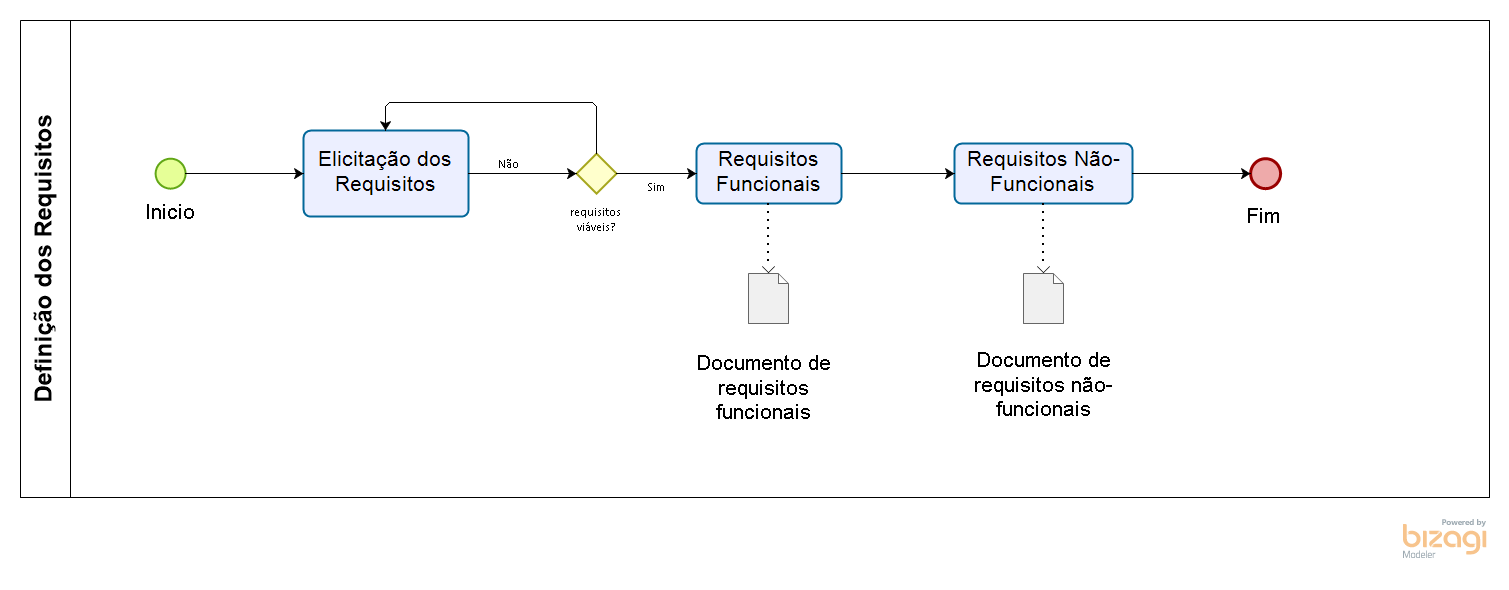
\includegraphics[width=1.0\textwidth]{figuras/elicitacaoDosRequisitos.png}
	\caption{Definição dos Requisitos. Fonte: Própria.}
	\label{img:definicao_requisitos}
\end{figure}

\subsubsection{Elicitação dos Requisitos}
\label{sec:elicitacao_requisitos}

\cite{sommerville} define a elicitação de requisitos como uma fase do projeto onde são extraídas informações do cliente sobre o que ele deseja que seja construído. É a fase em que o profissional de TI entende a necessidade do cliente e o orienta. É o momento de conversa com o usuário, de sentimento sobre o que este espera que seja entregue a ele. Na elicitação de requisitos são percebidas as necessidades do sistema e as características que esse sistema deve ter. Dentre todas as técnicas dentro da literatura, foram selecionadas duas como condidatas a serem usadas no projeto:

\begin{itemize}
    \item Entrevista
    \item Observação
\end{itemize}

\subsubsubsection{Entrevista}
\label{sec:entrevista}

Segundo \cite{sommerville}, as entrevistas podem ser formais ou não, mas fazem parte da maioria dos processos de engenharia de requisitos. Nas entrevistas, é realizada pela equipe de engenharia de requisitos perguntas aos \textit{stakeholders} sobre o sistema em vigor e o que será desenvolvido. A partir dessas perguntas surgem os requisitos.

As entrevistas podem ser de dois tipos: fechadas e abertas. Nas entrevistas fechadas, os \textit{stakeholders} respondem perguntas um conjunto de perguntas pré-definidas. Já nas entrevistas fechadas, são realizadas perguntas abertas sobre o sistema, e é nesse tipo de entrevista em que ocorre uma melhor compreensão das necessidades dos \textit{stakeholders}.  

\subsubsubsection{Observação}
\label{sec:observacao}

\cite{sommerville} define observação como uma técnica que pode ser usada para compreender os processos operacionais e ajudar a extrair os requisitos de apoio para esses processos. O trabalho do dia a dia é observado e são feitas anotações sobre as tarefas reais em que os partici­
pantes estão envolvidos. O valor da observação é que ela ajuda a descobrir requisitos implícitos do sistema que refletem as formas reais com que as pessoas trabalham, em vez de refletir processos formais definidos pela organização.

\subsubsection{Requisitos Funcionais}
\label{sec:requisitos_funcionais}

Os requisitos funcionais descreve o que o sistema deve de fato ser. Requisitos funcionais podem ser tão específicos quanto necessário,por exemplo, podem ter sistemas com requisitos funcionais gerais e outros que além de refletir os sistemas, também abrangem as formas de trabalho de uma organização. Requisitos funcionais de um sistema deve ser completo, isso quer dizer que todos os serviços requisitados pelo usuário devem ser definidos.

\subsubsection{Requisitos Não-Funcionais}
\label{sec:requisitos_nao_funcionais}

Requisitos não-funcionais são requisitos que são relacionados as propriedades do sistema como confiabilidade, tempo de espera, desempenho, segurança e até restrições do sistema. Requisitos não-funcionais podem possui tanta relevância quanto os requisitos funcionais, pois em uma reunião de levantamento de requisitos, o cliente sonha o mundo e não está atento se os recursos os próprios recursos e os recursos da emprega conseguem atender ao requisito. Um requisito não-funcional não atendido pode inclusive inutilizar um projeto. Exemplo disso é caso um sistema de uma aeronave não consiga atingir a confiabilidade necessária, não será dado o certificado de segurança para operar, sendo assim a aeronave não poderá voar.

\subsection{Linguagem de Software}

Linguagem de programação são instruções passadas de maneira que o computador entenda e apresente um retorno. Existem diversas linguagens de programação, desde a mais baixo a alto nível.

Linguagens de \textit{software}, como também podem ser chamadas, são divididas em duas frentes: \textit{front-end} e \textit{back-end}. Ambas serão explicadas nos tópicos a seguir.

\subsubsection{Front-end}
\label{sec:front-end}

A programação de um \textit{software} pelo ponto de vista do \textit{front-end} é a visão final do usuário com o sistema. \textit{Front-end} é a responsável pela interação do usuário com o sistema e essa interação é dada a partir de telas/páginas. Existem diversos tipos de \textit{frameworks} que auxiliam os desenvolvedores a trabalhar com essa frente, como:

\begin{itemize}
    \item \textit{Bootstrap
    \item Materialize
    \item React
    \item Angular 4}
\end{itemize}

\subsubsection{Back-end}
\label{sec:back-end}

A programação \textit{back-end} possui as responsabilidades de receber os dados pelo \textit{React}, que é o \textit{front-end} deste projeto, possui o dever de tratar os dados, valida-los e fomentá-los a visão do usuário.

Existem diversas linguagens \textit{back-end} que auxiliam os desenvolvedores a trabalhar em uma linguagem que o computador entende, como:

\begin{itemize}
    \item \textit{Python Django-Rest
    \item Java
    \item Ruby on Rails
    \item PHP}
\end{itemize}

\subsubsection{Arquitetura de Software}

A arquitetura de \textit{software} é como o sistema deve ser organizado com a estrutura geral do projeto. A arquitetura possui um valor alto dentro da construção de um \textit{software}, pois nela se tem o elo entre o projeto e a engenharia de requisitos. Possui o dever identificar os principais componentes estruturais no sistema e o relacionamento entre eles.

\subsubsection{Model-View-Controller}
\label{sec:mvc}

O padrão arquitetural MVC é responsável de responsabilidades em camadas. A primeira é \textit{Model}(modelo), que é responsável pela manipulação de dados, ou seja, leitura, escrita de dados e também suas validações é de responsabilidade da Model. A segunda camada é a \textit{View}(visão), que possui a responsabilidade de interação com o usuário. Por último se tem a \textit{Controller}(controladora), responsável por receber as aquisições do usuário. A controller também tem o dever de disponibilizar os dados para a \textit{view} e assim ocorrer a interação com o usuário.

\section{A Instituição}

Tendo a justificativa para o projeto no tópico \ref{sec:justificativa}, seguida do problema de pesquisa (\ref{sec:problema_de_pesquisa}) e os objetivos descritos no tópico \ref{sec:objetivos}, se tem a necessidade de escolher alguma empresa que será usada como caso de estudo para o projeto, no caso foi definido o NMIL (Núcleo de Modernização da Informação Legislativa), um setor localizado no Senado Federal Brasileiro.

\subsection{Senado Federal}

As funções do Senado Federal são exercidas pelos senadores da República, que são eleitos segundo o princípio majoritário para representarem os estados e o Distrito Federal. Cada estado e o Distrito Federal elegem três senadores para um mandato de oito anos. A renovação da representação se dá a cada quatro anos, alternadamente, por um e dois terços. Cada senador é eleito com dois suplentes.

A Estrutura Administrativa compreende a formação das unidades do Senado, suas
atribuições, responsáveis e formas de contato.

A Administração tem como ênfase os compromissos com o Parlamento; com excelência na prestação de serviços públicos; com qualidade de vida dos colaboradores; com a igualdade; com a livre disseminação de ideias; com a transparência; com a responsabilidade na utilização
de recursos públicos; com a ustentabilidade; com a acessibilidade; com a memória do Senado; e com a comunidade. Na figura \ref{img:organograma_senado} pode ser visualizado o organograma organizacional do Senado Federal com suas casas e secretárias.

\begin{figure}[H]
	\centering
	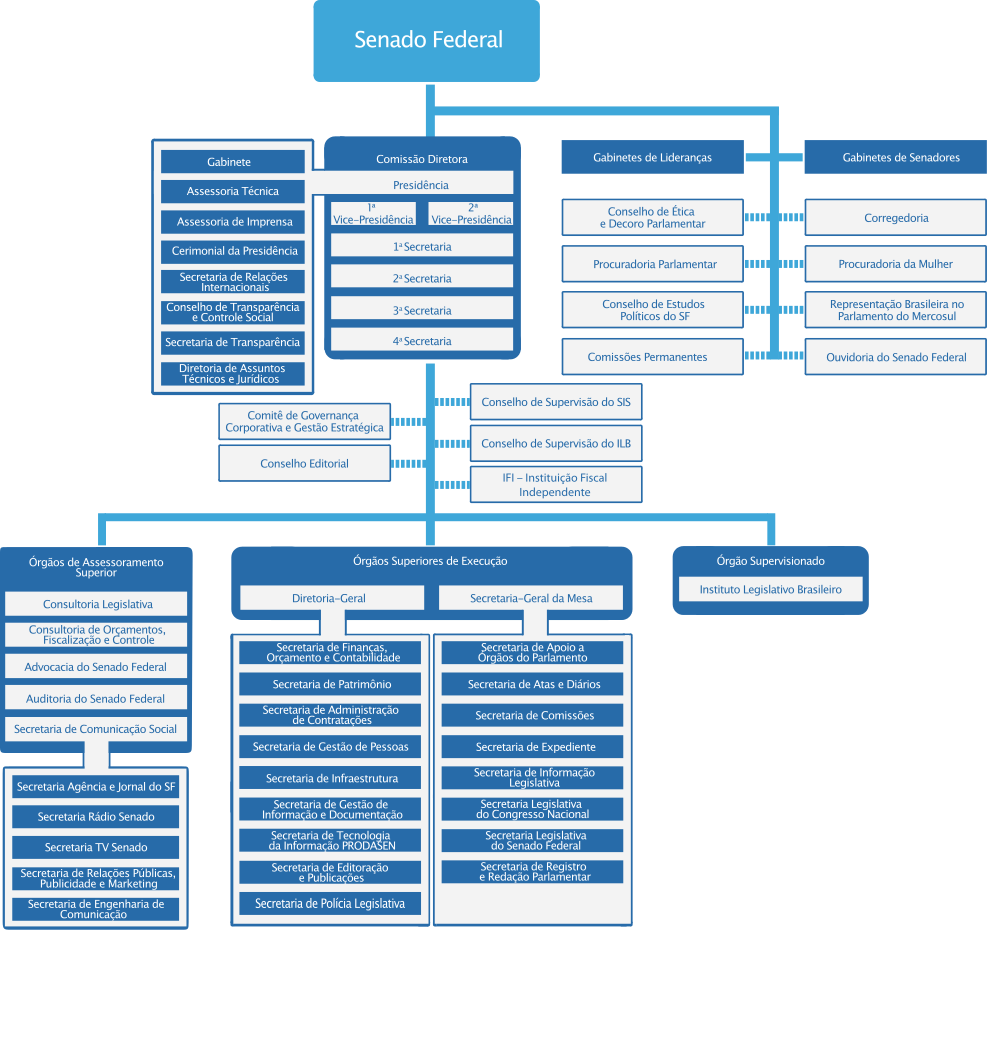
\includegraphics[width=0.8\textwidth]{figuras/organograma_senado.png}
	\caption{Organograma Senado Federal. Fonte: \cite{organograma_senado}.}
	\label{img:organograma_senado}
\end{figure}

\subsection{NMIL}

A Comissão Diretora é composta pelo Presidente, dois Vice-Presidentes e quatro
Secretários. A composição muda a cada dois anos, correspondentes a uma legislatura. É de responsabilidade da Comissão a direção da casa, designando atividades às unidades que dão suporte.

Essas unidades são: Secretaria Geral da Mesa (SGM), representante da atividade fim da casa; e Diretoria Geral (DGER), que, representa as atividades meio da casa. As duas contam com secretarias, às quais delegam atividades exigidas pelo Presidente.

Quando o Presidente da Comissão Diretora necessita de apoio tecnológico, delega esta
atividade à SGM, que, ao receber o problema, começa a definir diretrizes estratégicas para a solução do problema. Após o término da definição das diretrizes, encaminha-as à Secretaria de Informação Legislativa (Sinfleg).

O diretor da Sinfleg atua como Gerente do Projeto, e conta com o apoio da equipe do
NMIL na administração do projeto.

A equipe do NMIL realiza reuniões com as áreas afetadas pelo projeto até conseguir
definir todos os requisitos para o produto que será gerado, após a definição, convoca uma reunião com o Gerente para entrega dos requisitos definidos. O Gerente analisa esses requisitos para saber se são viáveis. Caso não sejam, pede ao NMIL novos requisitos e, só após receber requisitos viáveis, aprova a proposta de solução.

O próximo passo é dado pelo NMIL, convocando reunião com a Secretaria de Tecnologia da Informação (Prodasen). Nesta reunião discute-se os requisitos aprovados e prepara-se o Termo de Abertura do Projeto (TAP). O TAP, deve ser encaminhado pelo NMIL ao Gerente para que este aprove o documento; caso não aprove, pede-se um novo, até que seja aprovado.

Após o Gerente aprovar o projeto, ele o apresenta ao Secretário Geral da Mesa, que é o representante da SGM, para uma aprovação final. O Secretário Geral da Mesa também pode pedir um novo projeto, mas se não for o caso, apenas o autoriza.

Dada a aprovação do Secretário Geral da Mesa, a equipe do Prodasen, responsável pela
construção do produto, dá início à construção do produto, fazendo as entregas de ambiente de homologação (definidas no TAP) ao NMIL, a fim de que este realize testes. Se forem encontrados erros, estes são listados e repassados ao Prodasen para que sejam reparados. Quando não há mais erros, o NMIL dá sua aprovação do produto. Em seguida o Prodasen termina sua parte do projeto e entrega o produto finalizado ao NMIL. O NMIL encaminha o produto ao
Gerente que autoriza o produto e apresenta-o ao Secretário Geral da Mesa.

O Secretário Geral da Mesa, após receber o produto, pode solicitar alterações ao NMIL,
que em seguida encaminha esta solicitação ao Prodasen. A equipe do Prodasen responsável pelo produto faz as alterações necessárias o encaminha de volta ao NMIL, passando pelo processo de teste e aprovação novamente até que o Secretário Geral da Mesa autorize a implantação.

Quando o Secretário Geral da Mesa autorizar a implantação, cabe ao NMIL apresentar
aos usuários o novo Sistema ou as atualizações em sistemas já existentes.

As figuras relacionadas ao mapeamento do processo que ocorre atualmente no NMIL, pode ser vistos no apêndice \ref{ch:figuras}, sendo as figura \ref{img:modelagemProcessoGeral1Parte1} e \ref{img:modelagemProcessoGeral1Parte2} como o processo de pedido da comissão diretora para um novo sistema passando pela SGM, Sinfleg, NMIL e por fim ao Prodasen. As figuras \ref{img:modelagemProcessoGeral2Parte1} e \ref{img:modelagemProcessoGeral2Parte2} se referem ao processo que o NMIL passa até conseguir atingir um sistema estável e que atenda ao pedida da comissão diretora.